\documentclass{standalone}

\usepackage{tikz,tikz-3dplot,pgfplots,xcolor}
\usetikzlibrary{arrows.meta,calc}

\usepackage{amsmath}

\newcommand{\derivative}[2]{\frac{\partial #1}{\partial #2}}
\newcommand{\dderivative}[2]{\frac{\partial^2 #1}{\partial {#2}^2}}
\renewcommand{\exp}[1]{\ {\rm exp}\left( {#1} \right)}
\newcommand{\ext}[1]{#1^{\rm ext}}
\newcommand{\red}[1]{#1_{\rm red}}
\newcommand{\redn}[1]{#1_{\rm red,n}}
\newcommand{\inve}[1]{#1^{e-1}}
\newcommand{\transpose}[1]{#1^{\top}}
\newcommand{\ue}[1]{\underline{#1}^{e}}
\newcommand{\eT}[1]{{#1}^{e \top}}
\newcommand{\uT}[1]{\underline{#1}^{\top}}
\newcommand{\uprime}[1]{\underline{#1}^{\prime}}
\newcommand{\uTprime}[1]{\underline{#1}^{\prime \top}}
\newcommand{\vect}[1]{{\bf{#1}}}
\renewcommand{\sin}[1]{\ {\rm sin}\left( {#1} \right)}
\renewcommand{\sinh}[1]{\ {\rm sinh}\left( {#1} \right)}
\renewcommand{\cos}[1]{\ {\rm cos}\left( {#1} \right)}
\renewcommand{\cosh}[1]{\ {\rm cosh}\left( {#1} \right)}


\newcommand{\BB}{\vect{B}}
\newcommand{\BBT}{\transpose{\vect{B}}}
\newcommand{\BBe}{\vect{B}^e}
\newcommand{\BBeT}{\eT{\vect{B}}}

\newcommand{\cc}{\vect{c}}
\newcommand{\CC}{\vect{C}}
\newcommand{\cce}{\vect{c}^e}
\newcommand{\CCe}{\vect{C}^e}
\newcommand{\CCei}{\vect{C}^e_i}
\newcommand{\ccek}{\vect{c}^e_{\rm k}}
\newcommand{\ccen}{\vect{c}^e_{\rm n}}
\newcommand{\ccenI}{\vect{c}^e_{\rm n+1}}
\newcommand{\cck}{\cc_{\rm k}}
\newcommand{\ccn}{\vect{c}_{\rm n}}
\newcommand{\ccnred}{\redn{\cc}}
\newcommand{\ccred}{\red{\cc}}
\newcommand{\CCred}{\red{\CC}}

\newcommand{\cdt}{\dot{c}}
\newcommand{\cdtue}{\ue{\dot{c}}}
\newcommand{\cie}{c_i^e}
\newcommand{\cprime}{c^{\prime}}
\newcommand{\cpprime}{c^{\prime \prime}}
\newcommand{\cu}{\underline{c}}
\newcommand{\cue}{\ue{c}}
\newcommand{\cceT}{\eT{c}}
\renewcommand{\rmd}{{\rm d}}

\newcommand{\FF}{\vect{F}}
\newcommand{\FFe}{\vect{F}^e}
\newcommand{\FFext}{\ext{\FF}}
\newcommand{\FFred}{\red{\FF}}

\newcommand{\jje}{\vect{j}^e}
\newcommand{\Je}{J^{e}}
\newcommand{\Jeinv}{\inve{J}}
\newcommand{\jprime}{j^{\prime}}

\newcommand{\KK}{\vect{K}}
\newcommand{\KKe}{\vect{K}^e}
\newcommand{\KKei}{\vect{K}^e_i}
\newcommand{\KKred}{\red{\KK}}

\newcommand{\LLe}{\vect{L}^{e}}
\newcommand{\LLeT}{\eT{\vect{L}}}
\newcommand{\Nel}{N_{\rm el}}
\newcommand{\Nen}{N_{\rm en}}
\newcommand{\Nie}{N_i^e}
\newcommand{\Nip}{N_{\rm ip}}
\newcommand{\NN}{\vect{N}}
\newcommand{\NNe}{\vect{N}^e}
\newcommand{\NNeT}{\eT{\vect{N}}}
\newcommand{\NNT}{\transpose{\vect{N}}}
\newcommand{\Omegae}{\Omega^{e}}
\newcommand{\vv}{\vect{v}}
\newcommand{\vvT}{\transpose{\vect{v}}}
\newcommand{\vve}{\vect{v}^e}
\newcommand{\vveT}{\eT{\vect{v}}}
\newcommand{\xxe}{\vect{x}^e}

\newcommand{\zzero}{\vect{0}}


\newcommand{\dx}{\rmd x}
\newcommand{\dxi}{\rmd \xi}
\newcommand{\dxDxi}{\derivative{x}{\xi}}
\newcommand{\dDt}{\frac{\partial}{\partial t}}
\newcommand{\Dt}{\Delta t}
\newcommand{\dcDx}{\derivative{c}{x}}
\newcommand{\dcDxi}{\derivative{c}{\xi}}
\newcommand{\dcDt}{\derivative{c}{t}}
\newcommand{\dccDt}{\derivative{\cc}{t}}
\newcommand{\dcceDt}{\derivative{\cce}{t}}
\newcommand{\ddcDDx}{\dderivative{c}{x}}
\newcommand{\djDx}{\derivative{j}{x}}
\newcommand{\dGDt}{\derivative{G}{t}}
\newcommand{\dphiDx}{\derivative{\varphi}{x}}
\newcommand{\ddphiDDx}{\dderivative{\varphi}{x}}
\newcommand{\dNieDx}{\derivative{\Nie}{x}}
\newcommand{\dvDx}{\derivative{v}{x}}
\newcommand{\ddvDDx}{\dderivative{v}{x}}
\newcommand{\dvDt}{\derivative{v}{t}}

\newcommand{\intl}{\int\displaylimits_{x=0}^{l}}
\newcommand{\intOmega}{\int\displaylimits_{\Omega}}
\newcommand{\intOmegae}{\int\displaylimits_{\Omegae}}
\newcommand{\intXi}{\int\displaylimits_{\xi=-1}^{1}}
\newcommand{\sumel}{\sum_{e=1}^{\Nel}}
\newcommand{\sumip}{\sum_{i=1}^{\Nip}}
\newcommand{\sumNen}{\sum_{i=1}^{\Nen}}



%\pgfplotsset{compat=1.18} 
\definecolor{gray0}{rgb}{0.98,0.98,0.98}
\definecolor{gray1}{rgb}{0.8,0.8,0.8}
\definecolor{gray2}{rgb}{0.7,0.7,0.7}

\begin{document}

  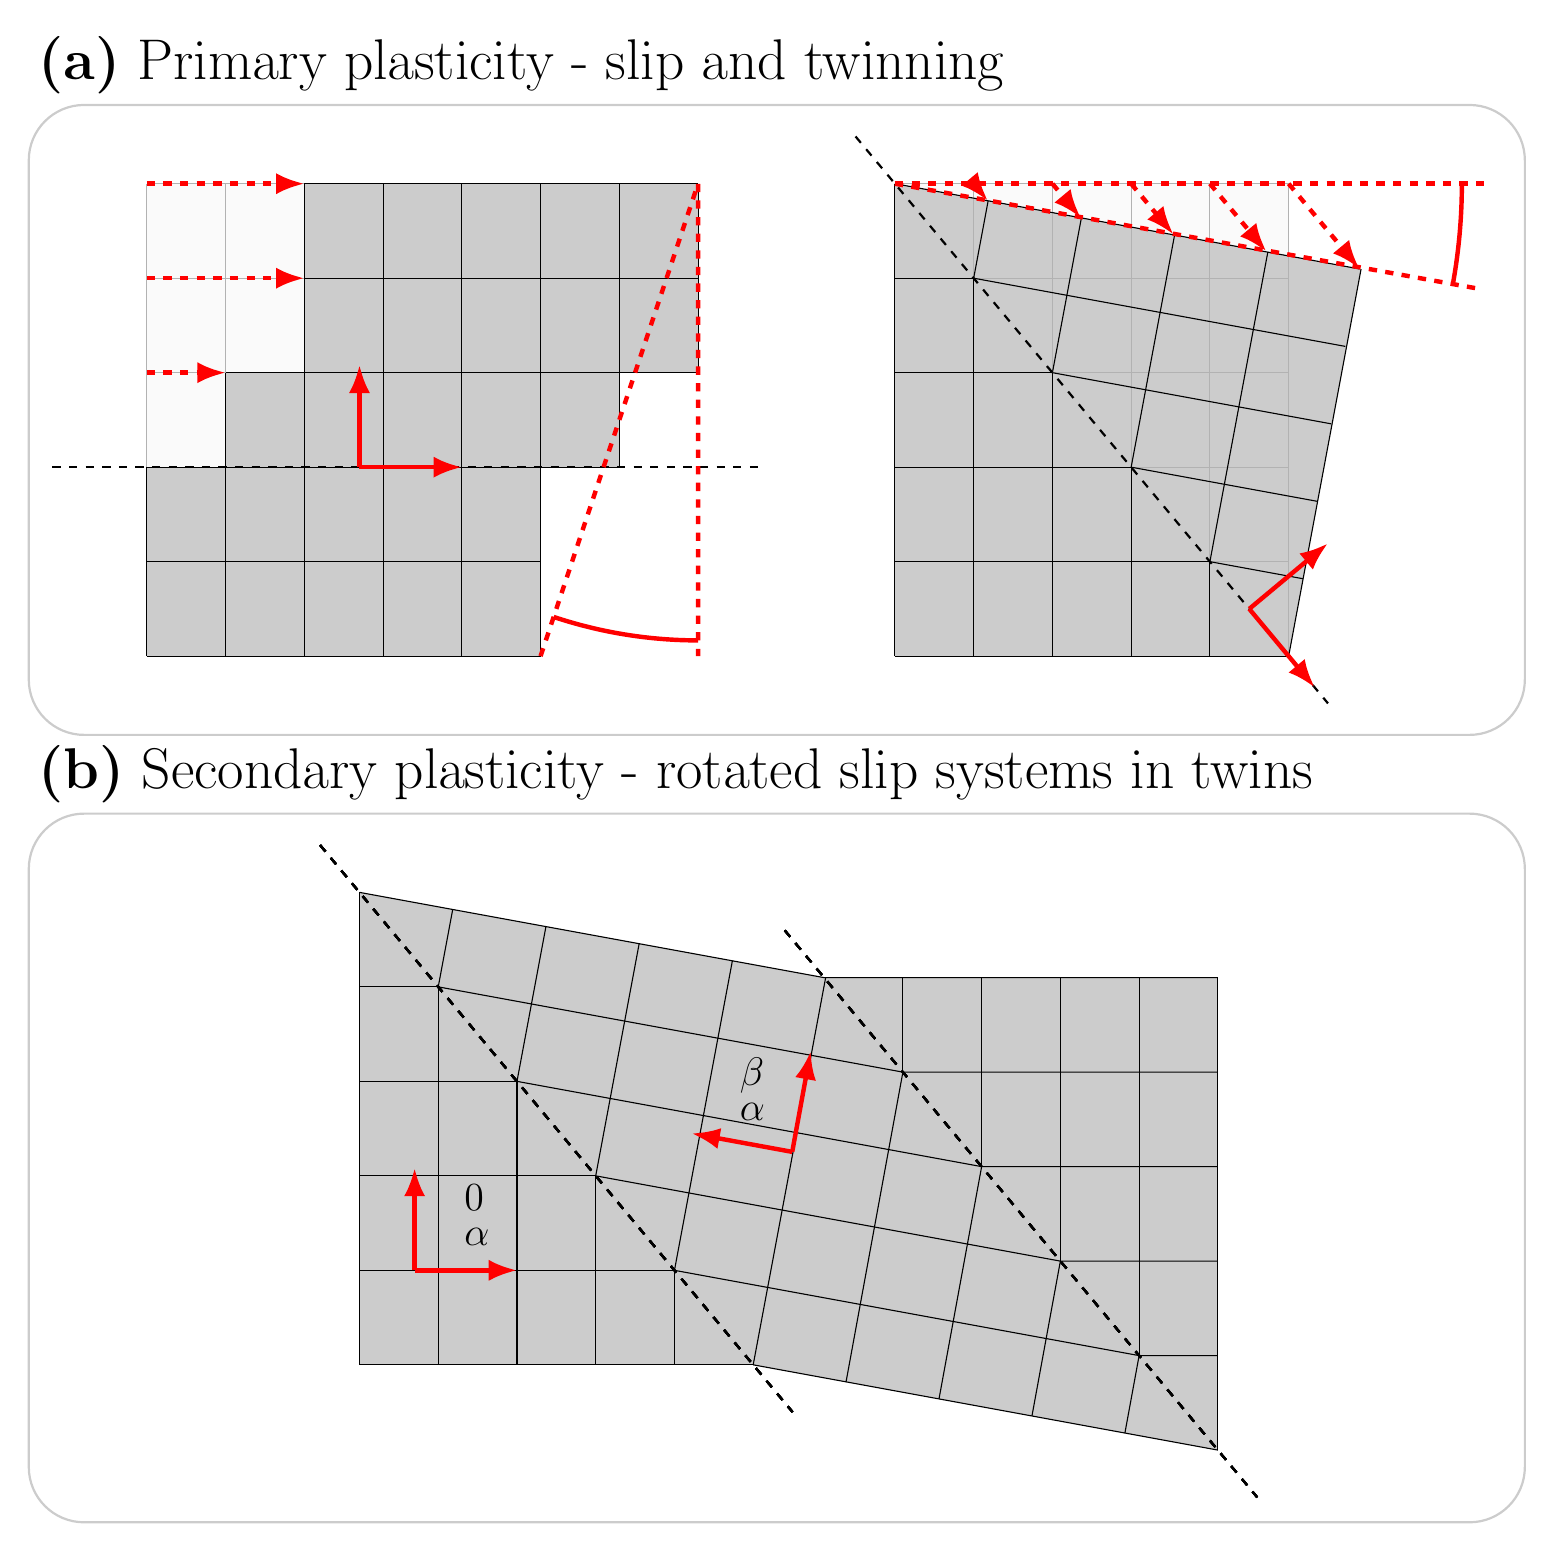
\begin{tikzpicture}[>=Latex]

    % \draw (-1,7) rectangle (18,-11);
    \draw[rounded corners=20pt,gray1,thick] (-1,7) rectangle (18,-1);
    \draw[rounded corners=20pt,gray1,thick] (-1,-2) rectangle (18,-11);
    \node[right] at (-1,7.5){\huge{\bf(a)} Primary plasticity - slip and twinning};
    \node[right] at (-1,-1.5){\huge{\bf(b)} Secondary plasticity - rotated slip systems in twins};

    \begin{scope}[shift={(10,0)}]
      \path[fill=gray0] (0,0) -- (5,0) -- (5,6) -- (0,6) -- cycle;
      \path[fill=gray1] (0,0) -- (5,0) --++ (79.4:5) -- (0,6) -- cycle;
      \foreach \x in {0,...,5}{
        \draw[gray2] (\x,0) -- (\x,6);
        \draw[gray2] (0,1.2*\x) -- (5,1.2*\x);
      }
      \foreach \x in {0,...,5}{
        \draw (\x,0) -- (\x,6-1.2*\x);
        \draw (0,1.2*\x) -- (5-\x,1.2*\x); 
        \draw (5-\x,1.2*\x) --++ (79.4:5-\x); 
        \draw (\x,6-1.2*\x) --++ (-10.4:6-1.2*\x);
      }
      \foreach \x in {1,...,5}{
        \draw[->,red,dashed,ultra thick] (\x,6) --++ (309.8:0.28*\x);
      }
      \path(0,6)--(5,0) coordinate[pos=-0.1](a) coordinate[pos=1.1](b) coordinate[pos=0.9](c);
      \draw[dashed,thick](a) -- (b);
      \draw[ultra thick,->,red] (c)--++(-50.2:1.3) node[above right,black] {\Huge$\dd$};
      \draw[ultra thick,->,red] (c)--++(39.8:1.3) node[above right,black] {\Huge$\nn$};
      \draw[dashed,ultra thick,red](0,6)--(7.5,6);
      \draw[dashed,ultra thick,red](0,6)--++(-10.2:7.5);
      \draw[red,ultra thick] (7.2,6) arc (0:-10.2:7.2);

    \end{scope}

    \begin{scope}[shift={(0.5,0)}]
      \path[fill=gray0] (0,0) -- (5,0) -- (5,6) -- (0,6) -- cycle;
      \path[fill=gray1] (0,0) -- (5,0) -- (5,2.4) -- (6,2.4) -- (6,3.6)--(7,3.6)--(7,6)--(2,6)--(2,3.6)--(1,3.6)--(1,2.4)--(0,2.4)--cycle;

      \draw[gray2] (0,0) -- (0,6);
      \draw[gray2] (1,0) -- (1,6);
      \draw[gray2] (2,0) -- (2,6);
      \draw[gray2] (0,3.6) -- (5,3.6);
      \draw[gray2] (0,4.8) -- (5,4.8);
      \draw[gray2] (0,6) -- (5,6);


      \draw (0,0) -- (5,0);
      \draw (0,1.2) -- (5,1.2);
      \draw (0,2.4) -- (6,2.4);
      \draw(1,3.6) -- (7,3.6);
      \draw (2,4.8) -- (7,4.8);
      \draw (2,6) -- (7,6);
      \draw (0,0) -- (0,2.4);
      \draw (1,0) -- (1,3.6);
      \draw (2,0) -- (2,6);
      \draw (3,0) -- (3,6);
      \draw (4,0) -- (4,6);
      \draw (5,0) -- (5,6);
      \draw (6,2.4) -- (6,6);
      \draw (7,3.6) -- (7,6);

      \draw[->,red,dashed,ultra thick] (0,3.6) --++ (1,0);
      \draw[->,red,dashed,ultra thick] (0,4.8) --++ (2,0);
      \draw[->,red,dashed,ultra thick] (0,6) --++ (2,0);
      \draw[dashed,thick] (-1.2,2.4) -- (7.8,2.4); 
      \draw[ultra thick,red,->] (2.7,2.4) --++ (1.3,0) node[above right,black]{\Huge $\dd$};
      \draw[ultra thick,red,->] (2.7,2.4) --++ (0,1.3) node[above,black]{\Huge $\nn$};
      \draw[dashed, ultra thick,red] (5,0)--(7,6)--(7,0);
      \draw[red,ultra thick] (7,0.2) arc (270:251.57:5.8);
    \end{scope}

    \begin{scope}[shift={(3.2,-9)}] 
      \path[fill=gray1] (0,0) coordinate(a) --++ (5,0) coordinate(b) --++ (-10.4:6) coordinate(c) --++ (0,6) coordinate(d) --++ (-5,0) coordinate(e) --++(169.6:6) coordinate(f) --cycle;

      \foreach \x in {0,...,5}{
        \draw (\x,0) -- (\x,6-1.2*\x) ;
        \draw (0,1.2*\x) -- (5-\x,1.2*\x); 
        \draw (5-\x,1.2*\x) --++ (79.4:5-\x); 
        \draw (\x,6-1.2*\x) --++ (-10.4:6) coordinate (cc) --+ (5-\x,0);
        \draw (cc) --+ (0,1.2*\x);
        \path (f)--(b) coordinate[pos=-0.1](aa) coordinate[pos=1.1](bb);
        \draw[dashed,thick] (aa)--(bb); 
        \path (e)--(c) coordinate[pos=-0.1](aa) coordinate[pos=1.1](bb);
        \draw[dashed,thick] (aa)--(bb); 
      }
      \foreach \x in {1,...,5}{
        \path (\x,6-1.2*\x) --++ (-10.4:6) coordinate (cc);
        \draw (cc) --+ (259.6:5-\x);
      }

      \node at (1.5,1.9){\huge $\MM_{\alpha}^{0}$};
      \draw[ultra thick,red,->](0.7,1.2)--++(1.3,0);
      \draw[ultra thick,red,->](0.7,1.2)--++(0,1.3);

      \node at (5,3.5){\huge $\MM_{\alpha}^{\beta}$};
      \path (b)--(e) coordinate[pos=0.55](aa);
      \draw[ultra thick,red,->](aa)--++(79.6:1.3);
      \draw[ultra thick,red,->](aa)--++(169.6:1.3);
      
    \end{scope}


  \end{tikzpicture}
\end{document}